\documentclass[a4paper,french]{report}
\usepackage{geometry,babel,graphicx,lineno,pdfpages}
\usepackage[T1]{fontenc}
\usepackage[utf8]{inputenc}
\usepackage[color links=true,link color=black]{hyperref}
\graphicspath{{./figs/}}
\makeatletter
%% meta function
\def\make@object#1{\expandafter\gdef\csname#1\endcsname{\object{#1}}}
\newcommand{\object}[1]{\texttt{#1}}
\make@object{forecast}
\make@object{bank}
\make@object{liquid}
\make@object{saving}
\make@object{operation}
\newcommand{\catForecast}[1]{\textsf{#1}}

%%% versions
\newcommand{\version}[3]{%
\setcounter{vmajor}{#1}
\setcounter{vmedium}{#2}
\setcounter{vminor}{#3}
}
\newcounter{vmajor}
\newcounter{vmedium}
\newcounter{vminor}
\newcommand{\theversion}{\thevmajor.\thevmedium.\thevminor}

\version{1}{0}{2}
\makeatother

\begin{document}

\author{Sylvain}
\date{Compilé le \today}
\title{Compta \theversion}

\pagenumbering{alph}
\maketitle

\pagenumbering{arabic}
\tableofcontents
\newpage

{\it%
Une comptabilité saine consiste à classer chaque opération
dont on veut garder une trace. Ce programme permet de
sauvegarder, classer et traiter des opérations de comptabilité
traditionnelle, c'est-à-dire des flux d'argent entre les liquidités,
un ou plusieurs compte en banques, un ou plusieurs compte épargnes,
le tout classer et traiter suivant un schéma prévisionnel.

Plus simplement, l'ensemble des dépenses que l'on opère se
classent dans différentes catégories, par exemple un loyer pourra être considéré
comme une dépense dans une catégorie \og Dépenses fixes\fg ou 
\og Administratif\fg, et les dépenses courantes pour la nourriture dans
une catégorie \og Vie courante\fg ou \og Inévitable\fg,\dots

Chacune de ces catégories va donc représenter une certaine somme
dépensée tous les mois, ce qui permet d'allouer à cette catégorie
une somme au début du mois. Une comptabilité comparera l'état
des dépenses effectuées à un certain moment avec les provisions
prévues, et donc permet de garder un \oe il sur l'état des
finances.

Ce programme se propose de tracer l'ensemble des flux d'argent,
en traitant l'ensemble des opérations par rapport à des prévisions,
les suivant entre le liquides, un ou des comptes en banque et comptes
d'épargne. Ainsi on a une estimation précise de l'argent restant dans le/les
compte(s) et en poche.
}


\chapter{Fonctionnement}
\label{chap:func}
\section{Les objets}
Une comptabilité se fait entre des comptes bancaires, des comptes d'épargne
associés et des liquidités. Les comptes d'épargne dépendent entièrement d'un
compte courant (appelé bancaire ici) auquel ils sont associés. Les flux d'argent
se passent entre l'extérieur et un compte (utilisation de carte bleue), un compte
et une liquidité (retrait d'un compte), un compte et une épargne associée
(voir Fig.~\ref{compta:comptes}).
\begin{figure}
\centering
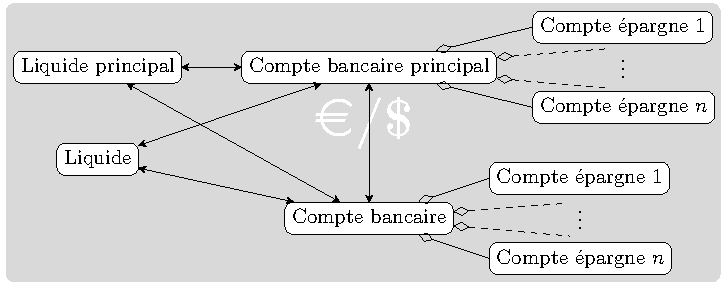
\includegraphics{entite}
\caption{\label{compta:comptes}Les comptes sont répartis entre comptes bancaires et
        comptes liquides. Tant qu'ils sont dans la même monnaie, ils peuvent tous
        interagir les uns avec les autres. Les comptes épargnes sont totalement gérés
        par le compte courant associé, rien ne peut en sortir/entrer sans passer
        par le compta bancaire.}
\end{figure}

Une tenue de comptabilité va consister à comptabiliser ces flux, les organiser
en catégories et comparer le total des flux avec des seuils. Il faut donc
un objet pour définir ces catégories et seuil: le prévisionnel.

\subsection{Prévisionnel}

Prévoir les dépenses peut se faire en les classant en catégories,
et en assignant à chacune d'elle un seuil à ne pas dépasser. 
La prédiction étant un art difficile,
et surtout lorsqu'il s'agit du futur\footnote{\og Prediction is very
difficult, especially about the futur.\fg\ \textsc{Niels Bohr}
(1885--1962)}, ce seuil peut se nuancer d'une certaine marge
pour le rendre flottant.
Ainsi chaque catégorie se caractérise par un nom, un seuil, mais
aussi une marge de man\oe uvre.

De plus, il est possible (et même fortement probable) qu'il existe des
opérations récurrentes tous les mois, typiquement des factures, 
un loyer, un prêt, etc. Ainsi il faut pouvoir ajouter
à certaines catégories des opérations qui, par hypothèse,
se passeront à un moment ou un autre dans le mois.

Un cran plus loin, il existe des opérations automatiques qui n'ont lieu qu'une
fois tous les deux mois, ou tous les $n$ mois de façon générale.
Il faut donc à chacune de ces opérations associer une période en
mois à laquelle il faut s'attendre à cette opération. Afin de bien
caractériser ce genre de comportement, il faut donc:
\begin{itemize}
\item une date de départ;
\item une date de fin;
\item une période;
\end{itemize}
pour une opération.

Au final, le prévisionnel est donc un ensemble de catégories, qui
peuvent contenir des sous-catégories afin de classer plus finement. Par
exemple on peut définir une catégorie \catForecast{Administratif}
qui regrouperait des transactions pour la nourriture, le transport,
etc. 

\`A cela, nous pouvons ajouter des opérations automatiques, par
exemple payer le loyer. Le loyer est payé tous les mois, il faut
donc s'y attendre s'il n'est pas passé. Un loyer ne dure que la période
pendant laquelle nous sommes locataires, autremement dit, une date de
début, une date de fin. De la même façon, la facture d'électricité doit
être payée, mais des fois tous les deux mois. Au final, notre catégorie
\catForecast{Administratif} peut se décrire ainsi:
\begin{itemize}
\item Transport, nourriture, etc;
\item \catForecast{Loyer}, de montant fixe, prévu tous les mois, pendant la période
                           de location;
\item \catForecast{Facture de gaz}, de montant prévu fixe, tous les deux mois,
                                    pendant la période dans un logement particulier.
\end{itemize}

\textit{In fine}, le prévisionnel est constitué de catégories, chacune pouvant
contenir des opérations attendues. Appelons \operation\ ces 
opérations attendues. Nous pouvons donc décrire le prévisionnel comme un 
ensemble de catégories contenant chacune un ensemble d'\operation s,
si par défaut une catégorie contient une \operation\ qui consiste
a attentre tout type de transaction dans ladîte catégorie, et possiblement
d'autres \operation s automatiques ou non, à attendre durant le mois.
La catégorie la plus petite est celle qui ne contient rien, ce qui
est équivalent à dire qu'elle ne contient qu'une \operation: l'\operation\
par défaut décrite plus haut.

Le but d'un prévisionnel est de pouvoir fournir chaque mois le montant total
et par catégorie, avec sa marge associée, à ne pas dépasser.

\subsection{Compte bancaire}
\subsubsection{Compte courant}
Un compte bancaire se compose d'un compte courant auquel
on associe une ou plusieurs épargnes. Un compte courant
a un historique et une monnaie.
\subsubsection{Compte épargne}
Un compte épargne a la monnaie de son compte courant associé, toutes
ses opérations sont liées au compte courant.
\subsection{Liquide}
Identique au compte bancaire, sans épargne.

\label{sec:object}

\chapter{Fichier d'entrée}
\section{Exemple complet}
\footnotesize
\begin{verbatim}
Longjumeau comptabilité
EUR
#Date           Category        Amount  Margin   sub cat, automatic, date start, date end
forecast        Prêt            627.71  0.00   Prêt taux 1, PA, 15/01/2012
forecast        Prêt            151.61  10.00   Prêt taux 2, PA, 15/01/2012
forecast        Assurance       300.00  150.00              , PNA
forecast        Téléphonie      2.00    0.00   Free Mobile, PA, 10/01/2012, 10/01/2015, 2
forecast        Téléphonie      4.77    0.00   OVH,         PA, 01/01/2012
forecast        Cadeaux         5.00    0.00   MSF,                PA, 01/01/2012
forecast        Cadeaux         6.00    0.00   AIDES,              PA, 01/01/2012
forecast        Cadeaux         7.00    0.00   CARE,               PA, 01/01/2012
forecast        Cadeaux         6.00    0.00   ADECE,              PA, 01/01/2012
forecast        Cadeaux         10.00   0.00   Secours Catholique, PA, 01/01/2012
forecast        Administratif   218.06  0.00   Appel de fonds Syndic,          PA, 01/01/2012
forecast        Administratif   30.00   0.00   virement Epargne Illyana,       PA, 01/01/2012
forecast        Administratif   2.40    0.00   Cotisation CNV Equipage Facile, PA, 01/01/2012
forecast        Administratif   5.40    0.00   Cotisation CNV Equipage 2,      PA, 01/01/2012
forecast        Administratif   3.62    0.00   Cotisation CNV Co-Equipage 2,   PA, 01/01/2012
forecast        Administratif   30.00   0.00   Assurance vie Sylvain,          PA, 01/01/2012
forecast        Administratif   500.00  150.00   , PNA
# Account       dependance         amount  start_date   name            , currency (if different)
bank            main               918.57  01/01/2012   BPVF
savings         BPVF                 0.00  01/01/2012   livret A enfants
savings         BPVF                 0.00  01/01/2012   Epargne Illyana
bank            other                0.00  01/01/2012   BoA             , USD
cash            main                 3.09  01/01/2012   liquide France
#Date           Category        Debit   Credit  Identifier  Liquide Operation
20/04/2012      Cadeaux         50.00   0.00    Bn      Chèque 239 mariage Olivia et JM
05/05/2012      Administratif   5.00    0.00    B       Youpi glop zork glups
16/05/2012      Administratif   82.00   0.00    B       Graaaak namok
16/05/2012      Administratif   24.26   0.00    B       Blurp
01/06/2012      Administratif   2.40    0.00    B       Cotisation CNV Equipage Facile
05/06/2012      Cadeaux         5.00    0.00    B       MSF
05/06/2012      Cadeaux         7.00    0.00    B       CARE
05/06/2012      Administratif   3.62    0.00    B       Cotisation CNV Co-Equipage 2
05/06/2012      Administratif   30.00   0.00    B       Assurance vie Sylvain
05/06/2012      Administratif   30.00   0.00    B       Plan Epargne Enfant Illyana
08/06/2012      Administratif   0.00    250.00  V       livret A enfants
08/06/2012      Administratif   25.00   0.00    V       liquide France
11/06/2012      Cadeaux         10.00   0.00    B       Secours Catholique
12/06/2012      Administratif   5.40    0.00    B       Cotisation CNV Equipage 2
12/06/2012      Téléphonie      6.95    0.00    B       OVH
13/06/2012      Administratif   402.66  0.00    V       BoA, 500 USD
13/06/2012      Administratif   0.00    500.00  V       livret A enfants
14/06/2012      Prêt            627.71  0.00    B       Prêt taux 1
14/06/2012      Prêt            151.61  0.00    B       Prêt taux 2
15/06/2012      Administratif   218.06  0.00    B       Appel de fonds Syndic
15/06/2012      Administratif   17.90   0.00    B       Appel de fonds Syndic pour clôture
20/06/2012      Cadeaux         6.00    0.00    B       ADECE
20/06/2012      Cadeaux         6.00    0.00    B       AIDES
20/06/2012      Téléphonie      2.00    0.00    B       Free Mobile
20/06/2012      Administratif   0.00    300.00  V       livret A enfants
\end{verbatim}
\normalsize


\section{Entête}
\linenumbers
\footnotesize
\begin{verbatim}
Longjumeau comptabilité
EUR
\end{verbatim}
\nolinenumbers

Les premières lignes sont simplement le titre pour la sortie \LaTeX\
et la monnaie à utiliser.


\section{Prévisionnel}
\linenumbers
\footnotesize
\begin{verbatim}
#Date           Category        Amount  Margin   sub cat, automatic, date start, date end
forecast        Prêt            627.71  0.00   Prêt taux 1, PA, 15/01/2012
forecast        Prêt            151.61  10.00   Prêt taux 2, PA, 15/01/2012
forecast        Assurance       300.00  150.00              , PNA
forecast        Téléphonie      2.00    0.00   Free Mobile, PA, 10/01/2012, 10/01/2015, 2
forecast        Téléphonie      4.77    0.00   OVH,         PA, 01/01/2012
forecast        Cadeaux         5.00    0.00   MSF,                PA, 01/01/2012
forecast        Cadeaux         6.00    0.00   AIDES,              PA, 01/01/2012
forecast        Cadeaux         7.00    0.00   CARE,               PA, 01/01/2012
forecast        Cadeaux         6.00    0.00   ADECE,              PA, 01/01/2012
forecast        Cadeaux         10.00   0.00   Secours Catholique, PA, 01/01/2012
forecast        Administratif   218.06  0.00   Appel de fonds Syndic,          PA, 01/01/2012
forecast        Administratif   30.00   0.00   virement Epargne ,              PA, 01/01/2012
forecast        Administratif   2.40    0.00   Cotisation CNV Equipage Facile, PA, 01/01/2012
forecast        Administratif   5.40    0.00   Cotisation CNV Equipage 2,      PA, 01/01/2012
forecast        Administratif   3.62    0.00   Cotisation CNV Co-Equipage 2,   PA, 01/01/2012
forecast        Administratif   30.00   0.00   Assurance vie,                  PA, 01/01/2012
forecast        Administratif   500.00  150.00   , PNA
\end{verbatim}
\nolinenumbers
\normalsize

Le prévisionnel (\textit{forecast} en anglais) permet la décomposition en catégories contenant
chacune une ou plusieurs opérations. En Fig.~\ref{forecast:example} est donnée la structure
du prévisionel en exemple.

\begin{figure}
\centering
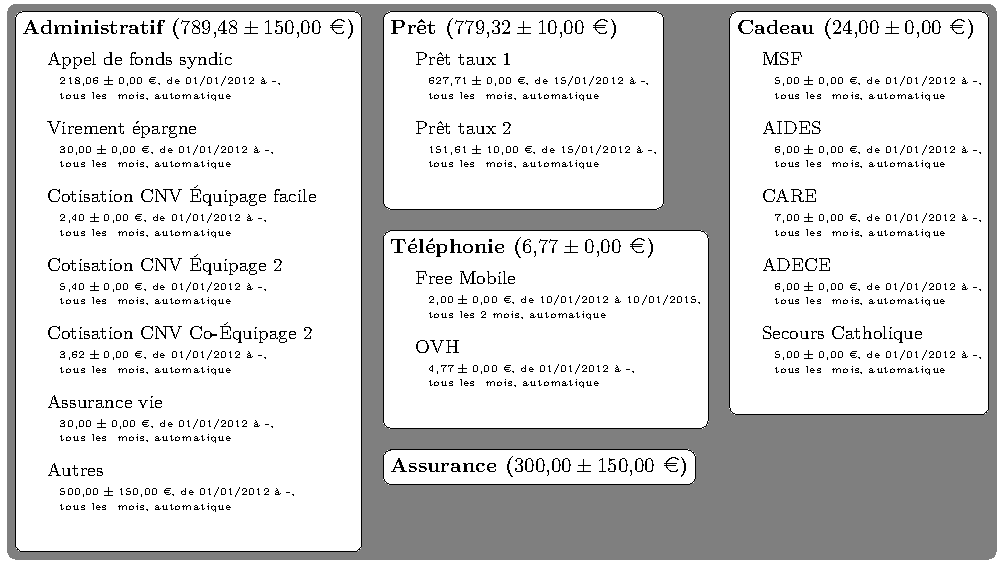
\includegraphics[width=\linewidth]{forecast_structure}
\caption{\label{forecast:example}Structure du prévisionnel de l'exemple.}
\end{figure}


\section{Comptes}
\linenumbers
\footnotesize
\begin{verbatim}
# Account       dependance         amount  start_date   name            , currency (if different)
bank            main               918.57  01/01/2012   BPVF
savings         BPVF                 0.00  01/01/2012   livret A enfants
savings         BPVF                 0.00  01/01/2012   Epargne Illyana
bank            other                0.00  01/01/2012   BoA             , USD
cash            main                 3.09  01/01/2012   liquide France
\end{verbatim}
\nolinenumbers
\normalsize


\section{Données}
\linenumbers
\footnotesize
\begin{verbatim}
#Date           Category        Debit   Credit  Identifier  Liquide Operation
20/04/2012      Cadeaux         50.00   0.00    Bn      Chèque 239 mariage Olivia et JM
05/05/2012      Administratif   5.00    0.00    B       Youpi glop zork glups
16/05/2012      Administratif   82.00   0.00    B       Graaaak namok
16/05/2012      Administratif   24.26   0.00    B       Blurp
01/06/2012      Administratif   2.40    0.00    B       Cotisation CNV Equipage Facile
05/06/2012      Cadeaux         5.00    0.00    B       MSF
05/06/2012      Cadeaux         7.00    0.00    B       CARE
05/06/2012      Administratif   3.62    0.00    B       Cotisation CNV Co-Equipage 2
05/06/2012      Administratif   30.00   0.00    B       Assurance vie Sylvain
05/06/2012      Administratif   30.00   0.00    B       Plan Epargne Enfant Illyana
08/06/2012      Administratif   0.00    250.00  V       livret A enfants
08/06/2012      Administratif   25.00   0.00    V       liquide France
11/06/2012      Cadeaux         10.00   0.00    B       Secours Catholique
12/06/2012      Administratif   5.40    0.00    B       Cotisation CNV Equipage 2
12/06/2012      Téléphonie      6.95    0.00    B       OVH
13/06/2012      Administratif   402.66  0.00    V       BoA, 500 USD
13/06/2012      Administratif   0.00    500.00  V       livret A enfants
14/06/2012      Prêt            627.71  0.00    B       Prêt taux 1
14/06/2012      Prêt            151.61  0.00    B       Prêt taux 2
15/06/2012      Administratif   218.06  0.00    B       Appel de fonds Syndic
15/06/2012      Administratif   17.90   0.00    B       Appel de fonds Syndic pour clôture
20/06/2012      Cadeaux         6.00    0.00    B       ADECE
20/06/2012      Cadeaux         6.00    0.00    B       AIDES
20/06/2012      Téléphonie      2.00    0.00    B       Free Mobile
20/06/2012      Administratif   0.00    300.00  V       livret A enfants
\end{verbatim}
\nolinenumbers
\normalsize


\appendix
\chapter{Sortie pdf de l'exemple}
\includepdf[pages=-]{./figs/Longjumeau_data}

\end{document}
